%%%%%%%%%%%%%%%%%%%%%%%%%%%%%%%%%%%%%%%%%
% University/School Laboratory Report
% LaTeX Template
% Version 4.0 (March 21, 2022)
%
% This template originates from:
% https://www.LaTeXTemplates.com
%
% Authors:
% Vel (vel@latextemplates.com)
% Linux and Unix Users Group at Virginia Tech Wiki
%
% License:
% CC BY-NC-SA 4.0 (https://creativecommons.org/licenses/by-nc-sa/4.0/)
%
%%%%%%%%%%%%%%%%%%%%%%%%%%%%%%%%%%%%%%%%%

%----------------------------------------------------------------------------------------
%	PACKAGES AND DOCUMENT CONFIGURATIONS
%----------------------------------https://texdoc.org/serve/xcharter-doc.pdf/0------------------------------------------------------

\documentclass[
	a4paper, % Paper size, specify a4paper (A4) or letterpaper (US letter)
	11pt, % Default font size, specify 10pt, 11pt or 12pt
]{CSUniSchoolLabReport}

\usepackage{titling}
\newcommand{\subtitle}[1]{%
  \posttitle{%
    \par\end{center}
    \begin{center}\large#1\end{center}
    \vskip0.5em}%
}

\addbibresource{sample.bib} % Bibliography file (located in the same folder as the template)

%----------------------------------------------------------------------------------------
%	REPORT INFORMATION
%----------------------------------------------------------------------------------------


%----------------------------------------------------------------------------------------

\begin{document}


%----------------------------------------------------------------------------------------
%	OBJECTIVE
%----------------------------------------------------------------------------------------
\section*{Information Visualisation Cousework 1 --- Brooklyn Mcswiney(ed20b3m)}
\begin{table}[h]
	\centering
	\caption{}
	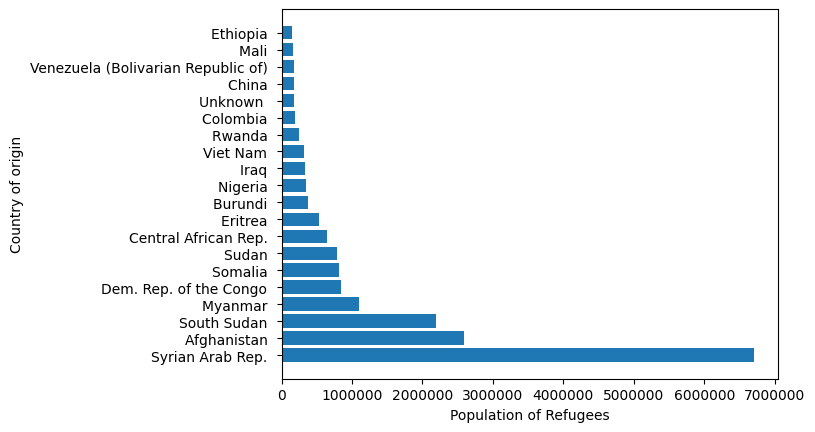
\includegraphics[width=0.6\textwidth]{population.png}
\end{table}
\begin{table}[h]
	\centering
	\caption{}
	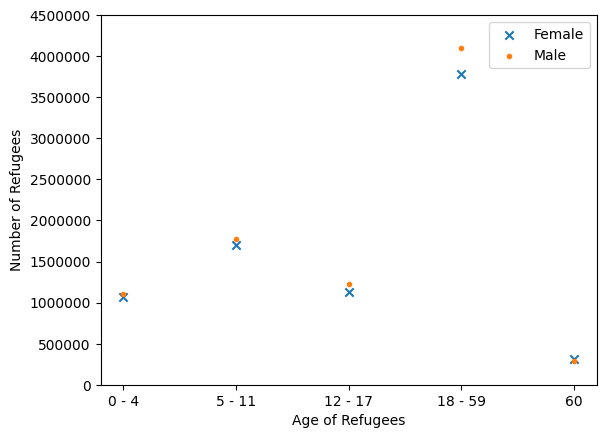
\includegraphics[width=0.6\textwidth]{demographics.png}
\end{table}

\begin{flushleft}
	Table 1 shows the top 10 places that refugees originate from. This shows that the Siryan Arab Republic
	has the most people leaving as refugees by a large factor.

	Table 2 shows the amount of refugees within certain age groups and separated by age. From this data 
	we can see that most refugees are between the ages of 18 and 59. We can also see that there are fractionally more 
	male refugees than female refugees.
\end{flushleft}
%----------------------------------------------------------------------------------------
%	BIBLIOGRAPHY
%----------------------------------------------------------------------------------------

%----------------------------------------------------------------------------------------

\end{document}